\documentclass[5p,sort&compress]{elsarticle}	
\newcommand{\RomanNumeralCaps}[1]
    {\MakeUppercase{\romannumeral #1}}
\makeatletter
\def\ps@pprintTitle{%
 \let\@oddhead\@empty
 \let\@evenhead\@empty
 \def\@oddfoot{\footnotesize\itshape
       \hfill\today}%
 \let\@evenfoot\@oddfoot}
\makeatother
\usepackage{dcolumn}
\usepackage[utf8]{inputenc}
\usepackage[T1]{fontenc}

\usepackage{textcomp}
\usepackage{lmodern}
\renewenvironment{abstract}{\global\setbox\absbox=\vbox\bgroup
\hsize=\textwidth\def\baselinestretch{1}%
\noindent\unskip\textbf{Abstract}
\par\medskip\noindent\unskip\ignorespaces}
{\egroup}
\usepackage{amsmath}
\usepackage{amssymb}
\usepackage{caption} %% figurer fugler
\usepackage{bm}
\usepackage{siunitx}
\sisetup{
exponent-product = \cdot,
output-decimal-marker  =  {.}, % komma-stil
separate-uncertainty = false, %true hvis du ikke vil ha usikkerhet i parentes
per-mode = symbol,
group-digits = false,
}
\usepackage{graphicx}
\renewcommand{\topfraction}{.85}
\renewcommand{\bottomfraction}{.7}
\renewcommand{\textfraction}{.15}
\renewcommand{\floatpagefraction}{.66}
\setcounter{topnumber}{3}
\setcounter{bottomnumber}{2}
\setcounter{totalnumber}{10}
\usepackage{flafter}
\usepackage{booktabs}
\usepackage{multirow}
\usepackage[colorlinks,linkcolor=pink]{hyperref}
\hypersetup{
    colorlinks=true,
    linkcolor=purple,
    filecolor=magenta,      
    urlcolor=cyan,
}
\usepackage{cleveref}
\usepackage{comment}
\usepackage{arydshln}
\usepackage[font=small,labelfont=bf]{caption}
\usepackage{subcaption}

% Dakrmode
\usepackage{xcolor}
% \pagecolor[rgb]{0.128, 0.128, 0.128}  %black
% \color[rgb]{0.848, 0.848, 0.848}  %grey

\usepackage{svg}
\urlstyle{same}


%%% LINK TIL DRIVE MED DATA

% https://drive.google.com/drive/folders/1--5J3TUoHqHPiAaSORvcn1TaKvSFUdGK?usp=sharing

%%%

\begin{document}
\begin{frontmatter}

  \title{TFE4575: Chemical methods for thin film deposition}
  %\title{Characterization of an Unknown Sample Using Scanning Electron Microscopy, Scanning Transmission Electron Microscopy, Energy Dispersive X-Ray Spectroscopy, Atomic Force Microscopy, and Raman Spectroscopy}

  \author[fysikk]{Brynjar Morka Mæhlummmmmmm}
  \author[fysikk]{Thord Niri Gjesdhal Heggren}


  \address[fysikk]{Department of Physics, Norwegian University of Science and Technology, 7491 Trondheim, Norway.}

  \begin{abstract}

    \noindent In this project, a Barium-Titanium-Oxide (BTO) thin film was made on a Si-Pt substrate using a sol-gel processing method. 
    The BTO film was made by first making a barium sol, and then combining it with a premade titanium sol. 
    This mixture was applied to the substrate using spin coating, followed by drying at 200°C and sintering at 700°C.
    The film was then characterized using an optical microscope, a stylus profilometer, and a scanning electron microscope.
    The optical microscope indicated that the film in general was homogenous, but that some artifacts were present.
    

  \end{abstract}


\end{frontmatter}

{ % Denne gjør table of contents pink i stedet for blå
\hypersetup{linkcolor=purple}
\tableofcontents
}

%%%%%%%%%%%%%%%%%%% THEORY %%%%%%%%%%%%%%%%%%
\section{Theory}

\subsection{Sol-Gel Synthesis Method}
\noindent This subsection is based on chapter 3 of B. L. Cushing \textit{et al.} review paper \textit{Recent Advances in the Liquid- Phase Synthesis of Inorganic Nanoparticles} \cite{solgel_review}.

In general, sol-gel processing combines small molecules to form a solid material.
This is done using a solution of precursors (the \textit{sol}) that forms a network of bound molecules (the \textit{gel}).
Traditionally, sol-gel processing only referred to the hydrolysis and condensation of alkoxide based precursor such as Si(OEt)$_2$ (tetraethyl orthosilicate), but today it refers to all processes using sol-gel.
The sol-gel synthesis method can be divided into the following six distinct steps.

Step (1): The formation of a stable solution of the alkoxide or solvated metal precursor.

Step (2): The gelation that results in the formation  an oxide- or alcohol-bridged network by polycondensation or polyesterification reactions.
This dramatically increases the viscosity of the solution.

Step (3):  The aging of the cell, also known as syneresis.
In this step, the gel network contracts and expulses the solution from the pores, and the reactions continue until the gel forms a solid mass.

Step (4): The drying of the gel where water and other volatile liquids are removed.
This step is complicated because it fundamentally changes the gel structure.
The drying process consists of four sub-steps: (i) the constant rate period, (ii) the critical point, (iii), the first falling rate period, and (iv) the second falling rate period.
The result is either termed a xerogel, if isolated by thermal evaporation, or an aerogel, if the solvent is extracted under supercritical conditions.

Step (5): Dehydration of the gel using high temperatures.
This removes surface-bound M-OH groups, thus stabilizing against rehydration.

Step (6): The densification and decomposition of the gel.
This makes the gel pores collapse, and all remaining organic species are volatilized.

\subsection{Chemistry of the Sols}

\noindent Using the sol-gel synthesis method, one can produce several types of materials.
One example of such a material is BTO (BaTiO$_3$), which can be made of a mixture of barium sol and titanium sol.
The following paragraph explains the components of these sols and what their functions are.

Barium sol can be made of a mixture of water, EDTA (Ethylenediaminetetraacetic acid), ammonia solution, barium nitrate, and citric acid.
Titanium sol can be made of a mixture of water, citric acid, Titanium isopropoxide, and ammonia solution.
The barium nitrate and the titanium isopropoxide are the sources of the barium and titanium, respectively.
Citric acid is a chelating agent, which means that it reacts with the metal ions to form stable, water-soluable metal complexes.
In the barium solution, EDTA is works as an additional complexing agent.
Finally, since the complex stability depends on the pH, the ammonia solution is used to for adjustments.

\subsection{Profilometer}

\noindent This subsection is based on \textit{nanoScience Instruments} optical profilometry manual \cite{profilometer_manual}.

Profilometers are instruments used to extract topographical data from a surface, e.g. surface morphology, step heights, and surface roughness.
This can either be done using a physical probe or by using light, and is then called stylus profilometey and optical profilometry, respectively.
Stylus profilometers typically gives a height profile along a line, while optical profilometers gives a height profile over an area.
All profilometers is built up of two main parts - a detector and a sample stage.
The detector determines where and how the measurements are taken, while the sample stage holds the sample.

In stylus profilometry, the stylus is physically in contact with the sample surface.
This is schematically shown in figure \autoref{fig:stylus_profilometer}.
At each x-y point, a force feedback loop measures the interactions between the stylus tip and the surface, and the z-value is extracted.
This method provides high vertical resolution, and is good for measuring step heights.
However, as there is physical contact, the surface can potentially be contaminated or damaged.
Also, the stylus tip size and shape influences the measurement, and thus limits the lateral resolution.

\begin{figure}[ht]
    \centering
    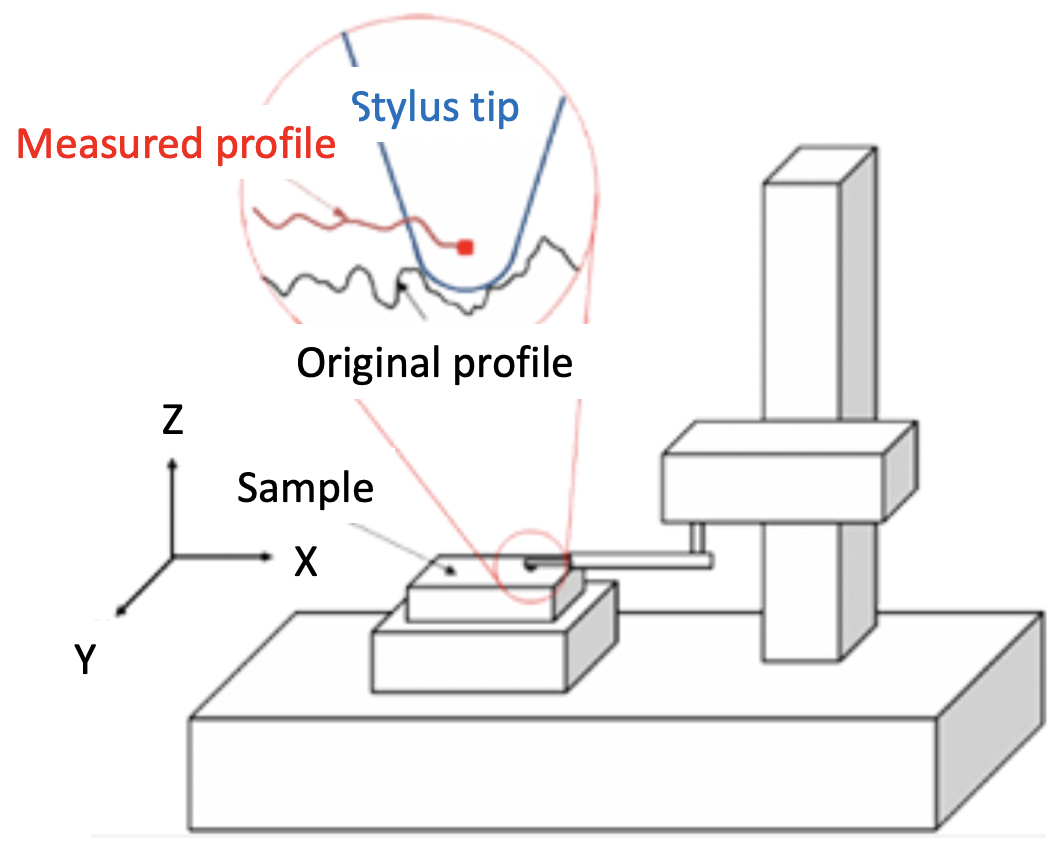
\includegraphics[width=0.45\textwidth]{figures/profilometer.png}
    \caption{Schematic illustration of a stylus profilometer. Figure adapted from \cite{profilometer_manual}.}
    \label{fig:stylus_profilometer}
\end{figure}


\subsection{Scanning Electron Microscope}

% short about the SEM and what contrast it gives.
\noindent The section on SEM is based on Goldstein chapter 1, 2, and 3 \cite{goldstein_scanning_2018}.
Scanning electron microscopes (SEM) are used for sample analysis, and the image contrast is due to the sample composition and topography.
Composition is given on elemental level with energy dispersive X-ray spectroscopy (EDS), or with Z-contrast imaging with backscattered electrons (BSE).
Topography is given primarily with secondary electrons (SE), and partly be achieved with backscattered electrons (BSE).
The Everhart Thornley Detector (ETD) combines data from the SE and BSE detectors to give a better image contrast \cite{T_Everhart_1960}.


% coating or not
SEM samples needs to be conductive, if not electrons will accumulate on the surface and the image will become distorted.
If the sample is not conductive enough, it can be coated with a thin layer of gold or carbon.
If a sample is partly conductive, a lower voltage can be used to get an image without distortion.

% seeing ferro electric domains in SEM
The SEM can be used to see ferroelectric domains structures in a sample, as illustrated in \autoref{fig:ferroelectric_domains_SEM_Hunnestad2019} from \cite{hunnestad_visualizing_2019}.
The image was taken on the SEM APREO at NTNU NanoLab with 1.5 kV and 50 pA, and gives an overview of the domains in the sample.


% insert figure ferroelectric_domains_SEM_Hunnestad2019.jpg
\begin{figure}[ht]
    \centering
    \includegraphics[width=0.45\textwidth]{figures/ferroelectric_domains_SEM_Hunnestad2019.jpg}
    \caption{
        Ferroelectric domains in an $ErMnO_3$ sample.
        The domains are visible as squiggly lighter and darker gray areas in the image.
        Image taken by Hunnestad and published in his master thesis in 2019 \cite{hunnestad_visualizing_2019}.
        Taken on the SEM APREO with EDT, 1.5 kV and 50 pA.
    }
    \label{fig:ferroelectric_domains_SEM_Hunnestad2019}
\end{figure}


%%%%%%%%%%%%%%%%%%% METHODS %%%%%%%%%%%%%%%%%%
\section{Methods}
\subsection{Barium sol}

In a beaker, 10 mL of DI water was heated to 60°C while being stirred with a magnet.
To this, 3.6893 g of EDTA and 7 mL of ammonia solution was added, and the solution was stirred until clear.
Then, 3.2676 g of Ba(NO$_3$)$_2$ and 4.8070 g of citric acid was added, and the solution was again stirred until clear.
Finally, about 3.5 mL of ammonia solution was added to achieve a pH of 7. 
This was verified using pH paper.
The final solution was then added to a 50 mL volumetric flask, and the volume adjusted to 50 mL with DI water.

\subsection{Titanium sol}

This titanium solution used in this project was premade by NTNU NanoLab.
However, the processing steps are included here for completeness and ease of replication.

In a beaker, 50 mL of DI water was heated to 60°C while being stirred with a magnet.
To this, 14.409 g of citric acid was added.
Then, 7.6 mL of titanium isopropoxide was added with a syringe.
The solution was then covered with parafilm and stirred overnight, until the solution was clear.
Finally, ammonia solution (30 \%) was added to adjust the pH to 7.

\subsection{Barium-titanium sol}

To make the barium-titanium sol (BTO



%%%%%%%%%%%%%%%%%%% RESULTS %%%%%%%%%%%%%%%%%%
\section{Results}
\subsection{Sample storage}
\label{sec:sample-storage}
\noindent The BTO sample was made during one session, stored in the toolbox for the course, and then characterized in a second session.
The synthesis was done on the 27th of September, and the sample was characterized on the 11th of October.
Unfortunately, the one-inch plastic sample box somehow opened during storage, and the sample was laying loose in the toolbox when it was taken out to be characterized.




\subsection{Optical Images}

\noindent Two images were obtained using an optical microscope.
First, a 5X magnification overview image was taken of one sample corner.
The result of this can be seen in \autoref{fig:optical_overview}.
Then, a 20X magnification image was taken of the middle of the sample.
The result of this can be seen in \autoref{fig:optical_20x}.

\begin{figure}[ht]
    \centering
    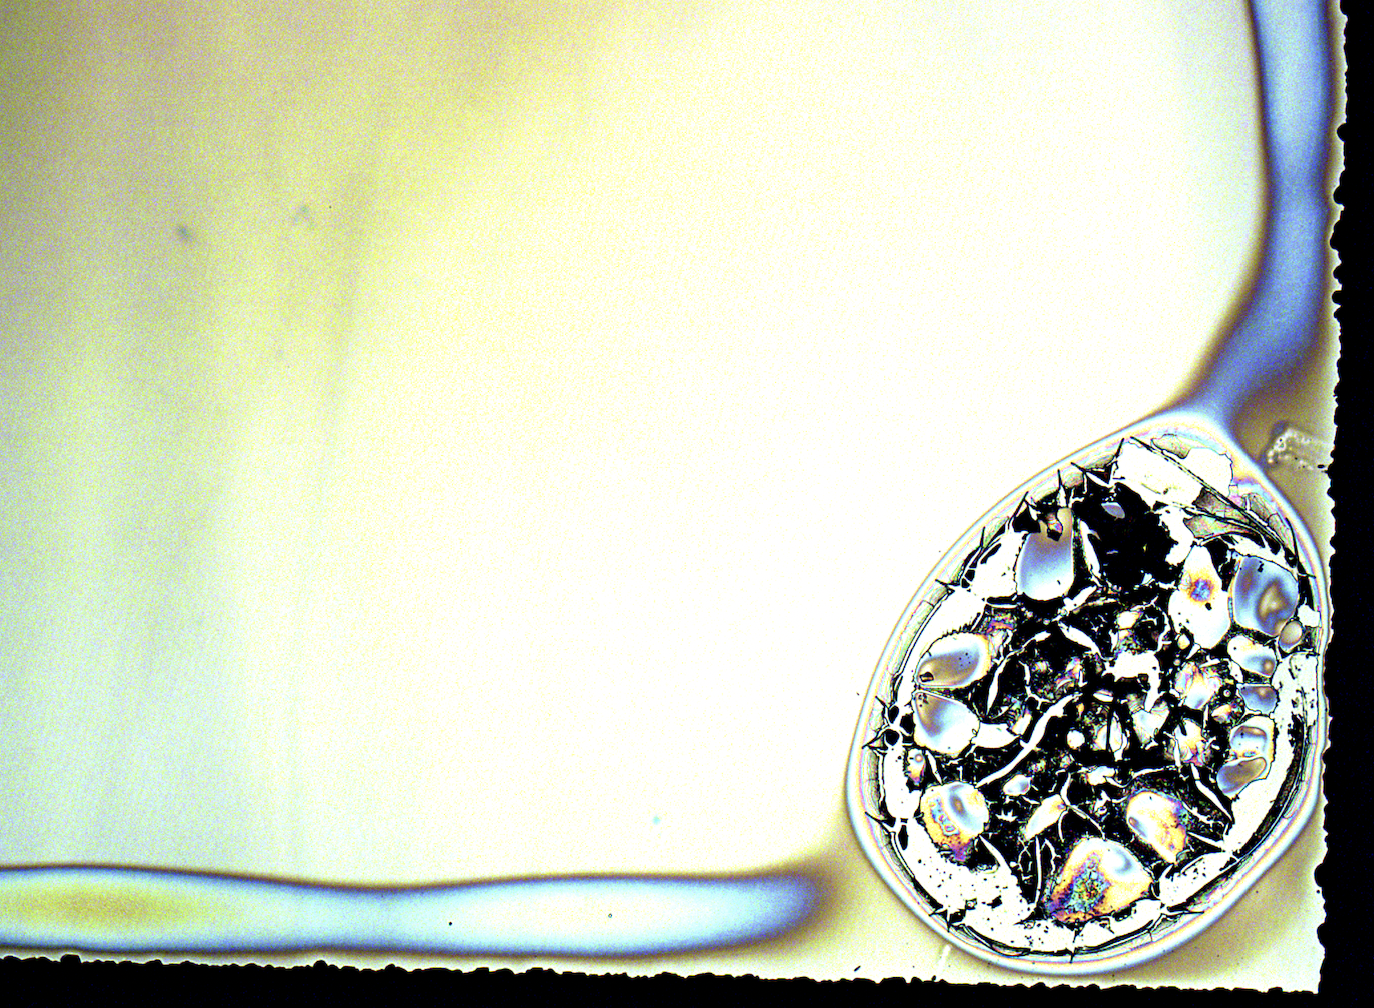
\includegraphics[width=0.45\textwidth]{figures/opt_corner.png}
    \caption{
        Optical overview image of one sample corner.
        The image was taken with a 5X magnification objective.
    }
    \label{fig:optical_overview}
\end{figure}

\begin{figure}[ht]
    \centering
    \includegraphics[width=0.45\textwidth]{figures/opt_mid.png}
    \caption{
        Optical 20X magnification image of artifacts in the middle of the sample.
        The image was taken with a 20X magnification objective.
    }
    \label{fig:optical_20x}
\end{figure}


% profilometer

\subsection{Profilometer}
\label{results:profilometer}

The profilometer data was acquired at three different locations on the sample.
The data is presented in \autoref{tab:profilometer} and \autoref{fig:profilometer}.
The only data processing done was flattening the data on the instrument computer, and later centering the data around zero, to make the data more comparable.

% table with profilometer data
\begin{table}[ht]
    \centering
    \caption{
        Profilometerdata in a table.
        The mean is zero because each data set is centered around zero.
        All measurements are 4000 \textmu m long.
        All numbers are in nm.
        Q1 and Q3 are the first and third quartile, respectively.
    }
    \begin{tabular}{ccccccc}
        Mean & Median & STD   & Min    & Max   & Q1     & Q3   \\
        \hline
        0.00 & -0.10  & 4.19  & -11.11 & 50.56 & -2.54  & 3.17 \\
        0.00 & -1.04  & 5.75  & -12.72 & 15.52 & -4.84  & 4.84 \\
        0.00 & 1.72   & 11.73 & -21.48 & 29.77 & -11.77 & 8.44 \\
    \end{tabular}
    \label{tab:profilometer}
\end{table}


% profilometer figure, filename figures/profilometer_graph.jpg

\begin{figure}[ht]
    \centering
    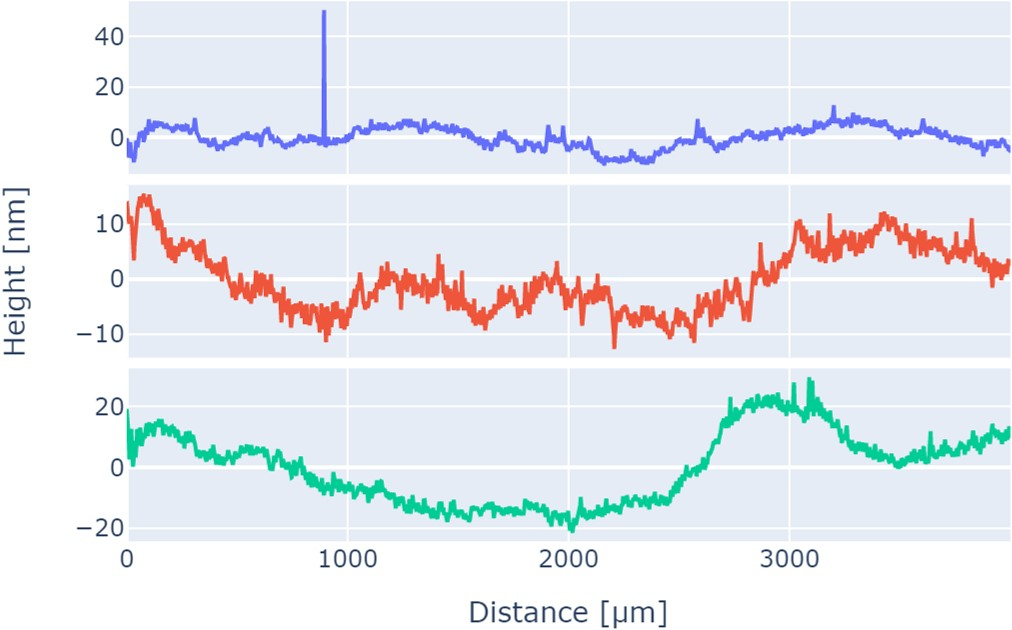
\includegraphics[width=0.45\textwidth]{figures/profilometer_graph.jpg}
    \caption{Profilometerdata showing scan 1, 2, and 3.
        Plotted with the mean centered around zero.
        The plots are with slightly different scales on the y-axis to include as much info as possible.
        Acquired at NTNU NanoLab.
    }
    \label{fig:profilometer}
\end{figure}



% SEM
\subsection{SEM images}
\label{results:SEM}

SEM images were acquired on the SEM APREO at NTNU NanoLab, without coating of the sample.
One of the engineers at NanoLab suggested that the sample would be conductive enough, and showed examples of SEM results from other ferroelectric thin films that were not coated, e.g. \cite{hunnestad_visualizing_2019}.
The examples used low voltage and low current, which was also used in this work.
The thickness of the film was only measured at the edge.

% SEM image of the corner
\autoref{fig:sem_high_res} shows an overview SEM image of a corner, which is the same area in the optical image in \autoref{fig:optical_overview}.
The image was taken with 3 kV and 50 pA, using the EDT detector to get both topography and z-contrast.
The scale bar is 250 \textmu m.

% SEM image of what might be pores
\autoref{fig:sem_overview} shows a closer SEM image of a part of the sample.
The image was taken with 5 kV and 0.1 nA, using the T2 SE detector, thus getting only topography contrast.
The scale bar is 5 \textmu m.
This image is of the edge, which is visible in the lower left corner.
Here the thickness is measured to be 670 nm, when assumed that the BTO thin film is only the darker top layer.

% SEM image of artifact which is 10 um long
\autoref{fig:sem_artifact} shows a close up SEM image of an artifact which is 15 \textmu m long and 5 \textmu m wide.
The image was taken with 5 kV and 0.1 nA, using the T2 SE detector, thus getting only topography contrast.
The scale bar is 10 \textmu m.

% SEM image filename figures/sem-overview.jpg
\begin{figure}[ht]
    \centering
    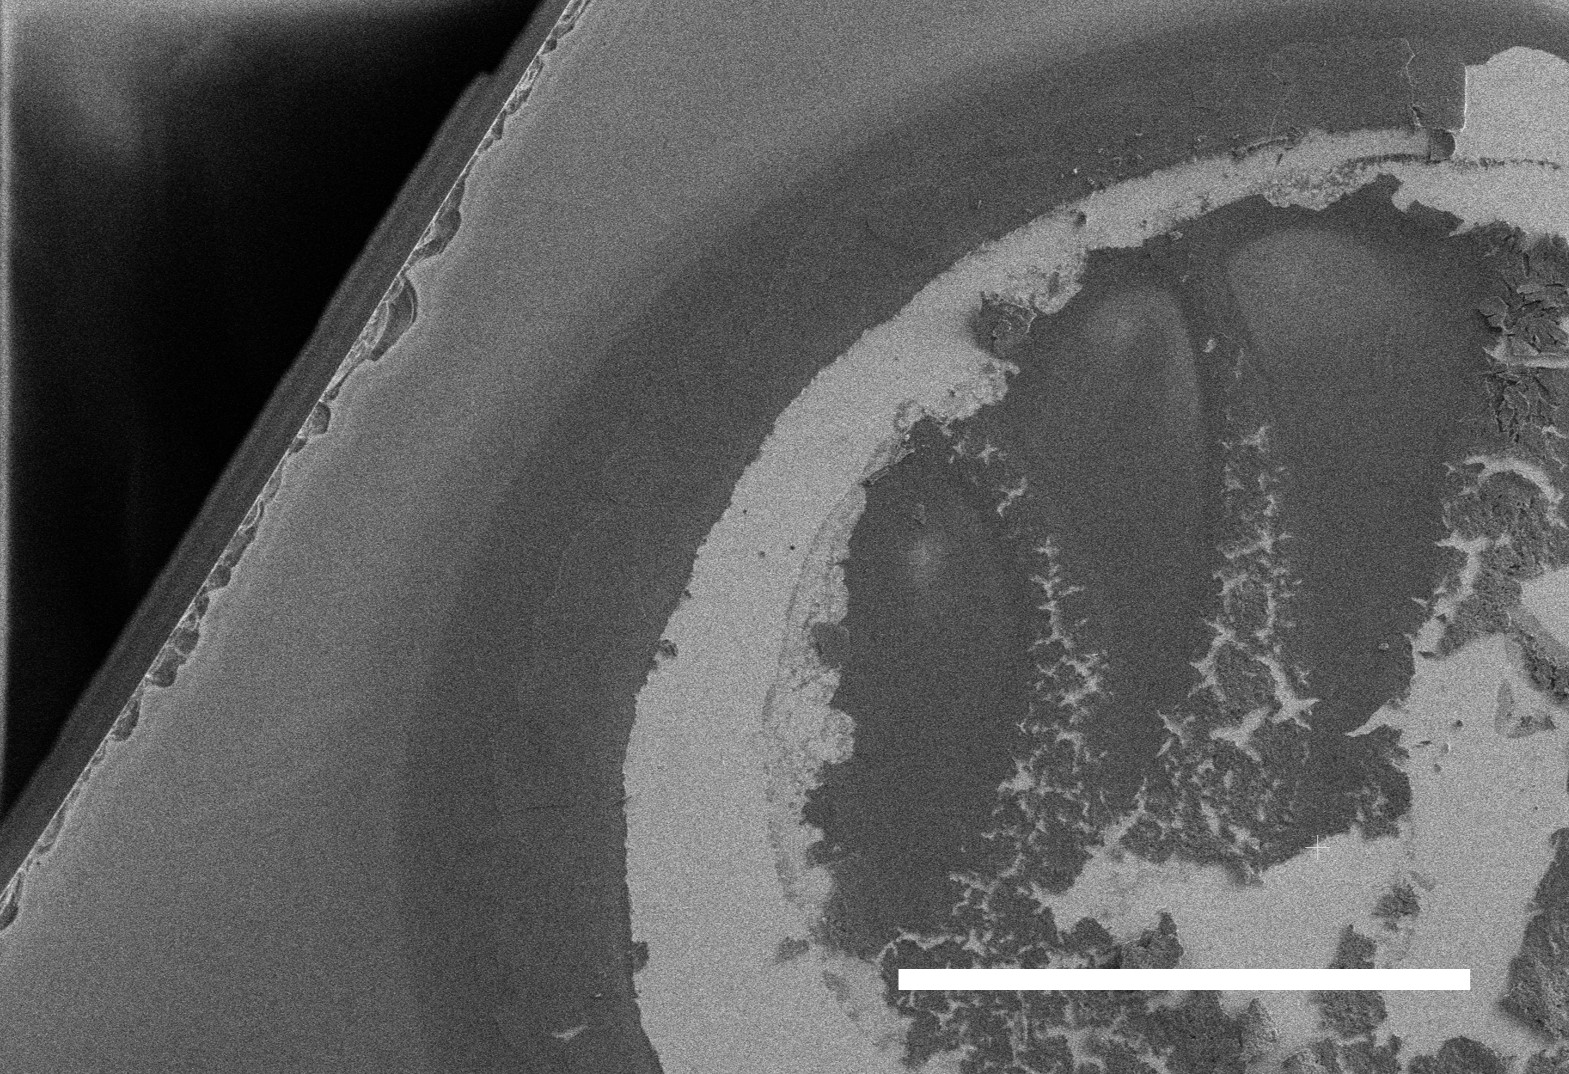
\includegraphics[width=0.45\textwidth]{figures/sem_overview_250um.jpg}
    \caption{Overview SEM image of a part of the sample.
        The scale bar is 250 \textmu m.
        3 kV, 50 pA, EDT detector, 3.9 mm WD, 200X magnification.
        Acquired at NTNU NanoLab.
    }
    \label{fig:sem_overview}
\end{figure}

% SEM image filename figures/sem-high-res.jpg
\begin{figure}[ht]
    \centering
    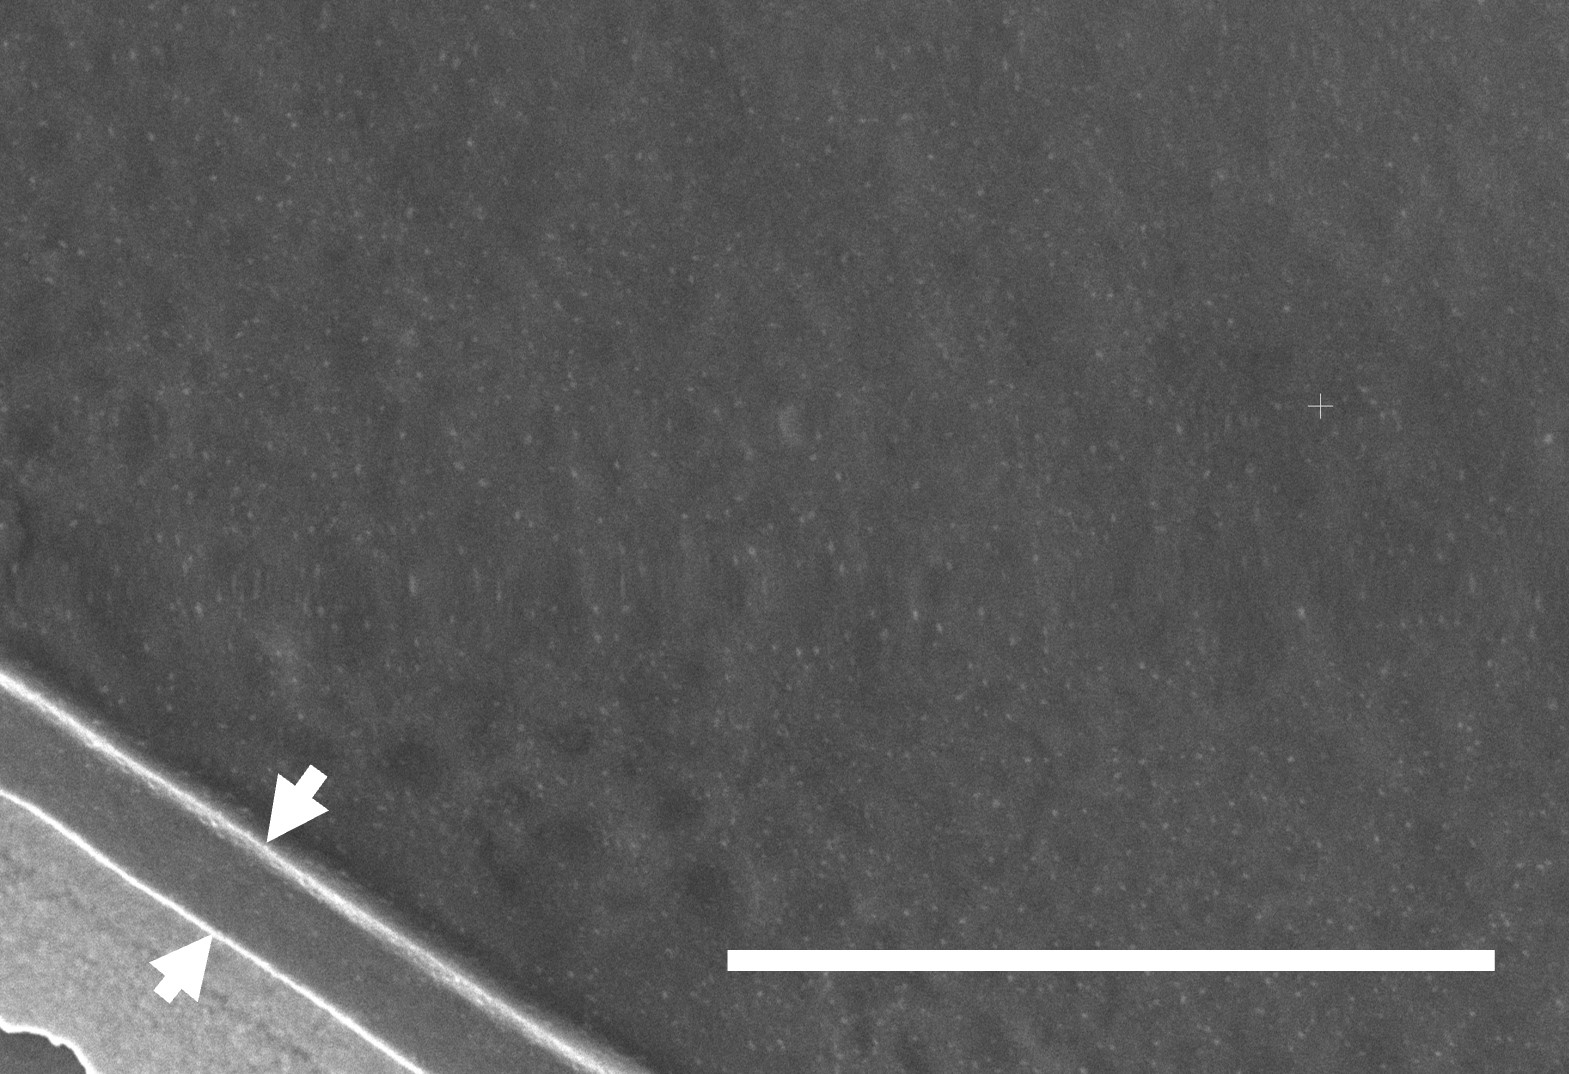
\includegraphics[width=0.45\textwidth]{figures/sem_high_res_5um.jpg}
    \caption{High resolution SEM image of the sample.
        The scale bar is 5 \textmu m.
        The edge is visible in the lower left corner, where the thickness is measured to be 670 nm.
        5 kV, 100 pA, T2 SE detector, 3.0 mm WD, 12000X magnification.
        Acquired at NTNU NanoLab.
    }
    \label{fig:sem_high_res}
\end{figure}

% SEM image artifact
\begin{figure}[ht]
    \centering
    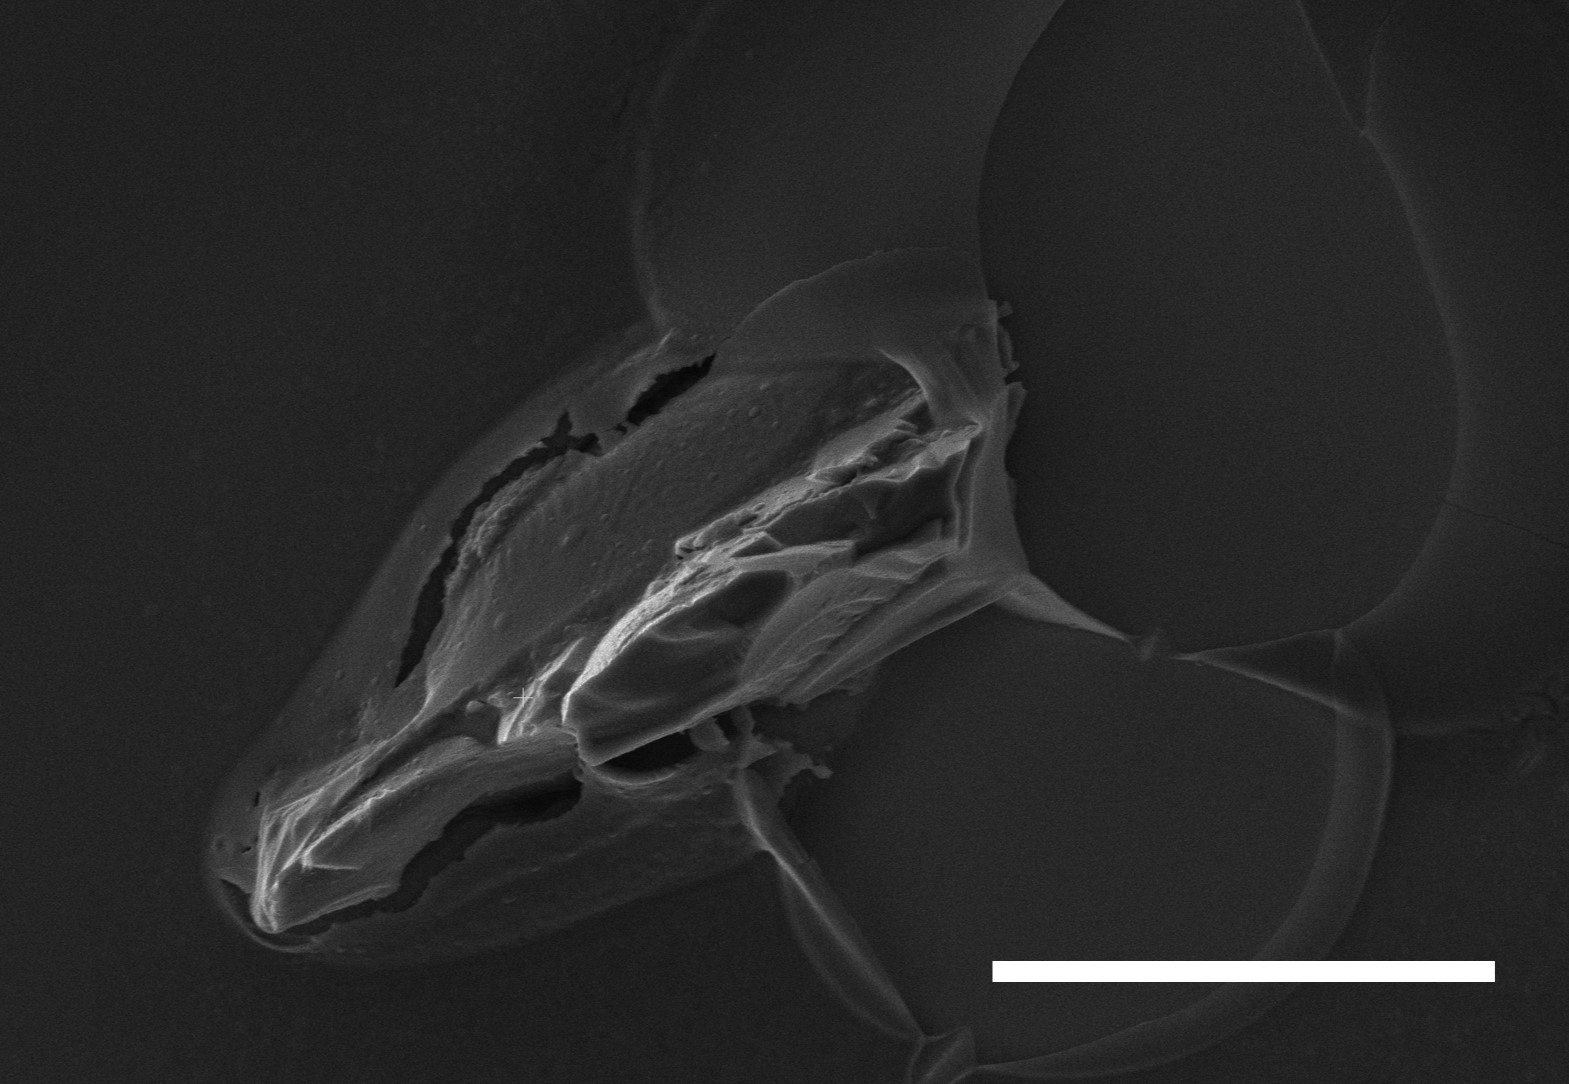
\includegraphics[width=0.45\textwidth]{figures/sem_artifact_10um.jpg}
    \caption{A close up SEM image of an artifact.
        The scale bar is 10 \textmu m.
        5 kV, 100 pA, T2 SE detector, 3.0 mm WD, 5000X magnification.
        Acquired at NTNU NanoLab.
    }
    \label{fig:sem_artifact}
\end{figure}


%%%%%%%%%%%%%%%%%%% DISCUSSION %%%%%%%%%%%%%%%%%%
\section{Discussion}

\subsection{Optical Images}

\noindent \autoref{fig:optical_overview} shows that visually, away from the substrate edges, the film appears to be homogenous.
The blue areas at the bottom and to the right could be due to a different film thickness in these regions.
Different thicknesses will reflect light differently and thus be another color.
The reason for this deviation might be due to bad spin coating or some edge effect during the heating steps.

In the same figure, there is a large, circular artifact.
Visually, this looks like the film has flaked off the substrate.
It is difficult to determine the exact reason why this happened.
One suggestion is that the adhesion between the film and the substrate was insufficient due to bad cleaning.
However, if this was the case, one could probably expect this to happen in other areas as well.

\autoref{fig:optical_20x} shows that artifacts were present at the regions that appeared homogeneously in the lower magnification image.
From the picture, it looks like there are two types of artifacts -  one blue circular and several black smudges.
The difference between them might be that the black ones lies \textit{on} the film, while the blue lays \textit{in} the film.
The reason for this difference may be related to when these artifacts arrived to the sample, where the blue ones are from before the film was dry.
It is possible that the black ones are a result of the bad sample storage.
However, with the information available from only the optical images, it is not possible to conclude on what these artifacts are and why they are there.

\subsection{Profilometer}

% flattness and roughness. STD is RMS which kinda is roughness
\noindent In general, the results from the profilometer shows that the film is relatively flat.
The STD of the three measurements is a way of quantifying the roughness of the film, and the values are low.
The mean values in \autoref{tab:profilometer} give that the STDs are $(4.19 + 5.75 + 11.73) \textnormal{ nm} / 3  = 7.22 \textnormal{ nm}$, which is not completely flat, but still not too rough. % $\frac{(4.19 + 5.75 + 11.73) \textnormal{nm}}{3}  = 7.22 \textnormal{nm}$
The quantiles are another way of quantifying the roughness of the film.
The Q1 and Q3 values are the 25th and 75th percentiles, respectively.
The difference between these two values is the interquartile range, which is a measure of the spread of the data.
The first measurement have a sharp artifact at around 900 \textmu m, but is also the flattest of the three measurements.
The second measurement have some smaller irregularities, but is still quite flat.
The third measurement have one large artifact between 2500 and 3500 \textmu m, but is also the roughest of the three measurements.
When plotting the three measurements on the same scale, the first and second measurements are very similar, while the third is more rough.

% potential pores
The profilometer data show potential signs of pores in the film.
There are some dips in the plotted data, which are ranging from 5 to 15 nm.
A dip this shallow is not large enough to be considered a pore, but it is still a sign of a potential pore.
It could be that the tip is too wide to detect pores, since the dips are around 10 \textmu m long.
The tip of the stylus is 12.5 \textmu m wide, so it is likely that the dips are too small to be detected.
The SEM data could potentially show if there are pores in the film.

% artifacts 1, the peak. peak and 
The profilometer data also show some artifacts.
The most obvious one is the peak at around 900 \textmu m in the first measurement.
This peak is 50 nm above the average and are 10 \textmu m long.
The artifact could be a contamination on top of the surface of the film, or it could be a contamination which was in the gel before the sintering.
The last possibility fits well with the SEM image of an artifact shown in \autoref{fig:sem_artifact}.

% artifacts 2, the deformation
A second artifact shown in the profilometer data is the deformation at around 2500 \textmu m in the third measurement.
This deformation has a bell shape and is 20 nm high and 1000 \textmu m long.
This artifact is probably a deformation since the optical and SEM images did not show any contamination that big.


\subsection{SEM}

% roughness in SE images.
\noindent The SEM images show that the film have a continuous surface, edge effects, some roughness, and potentially some pores.
The roughness is visible in the high resolution images as darker craters in \autoref{fig:sem_high_res} and as small "bubbles" in \autoref{fig:sem_artifact}.
The potential pores are visible as small lighter dots in the high resolution images in \autoref{fig:sem_high_res}.

% surface cracked or smooth, and edge/corner effects
The overview in \autoref{fig:sem_overview} shows clearly that the surface at the corner is cracked or flaked.
The defect is most likely flaking and not cracking, as the defects are not sharp.
The different gray levels are probably due to the z-contrast, showing the exposed wafer beneath the film as a lighter gray.
The area is the same as in the optical image in \autoref{fig:optical_overview}, and the SEM image shows that the film is not homogenous in this area.
The high resolution SEM image in \autoref{fig:sem_high_res} is also taken at an edge, but not at a corner.
The high resolution image show that the edge effects are not as severe on the whole surface as in the overview image.
The reason for a worse edge effect at the corner could be that the spin coating usually yields the worst results in the corners, or it could just be handling of the sample.
While handling the sample, the edges are more exposed, and it is easiest to pick up the sample from the corner.

% thickness
The thickness of the sample was only measured one place, and that was on the edge in \autoref{fig:sem_high_res}.
An edge it not necessarily the best place to measure the thickness, but it does give an indication of the thickness.
The thickness here was measured to be 670 nm.


% pores we might see
The potential pores visible in the high resolution SEM image as lighter dots could also be the film defect called pinholes.
Pinholes are small holes in the film, which are caused by dirt and impurities in the gel.
With the data available, it is difficult to conclude whether the dots are pores or pinholes.
Potential pores could have remained after the sintering process, where organic species were driven out of the film as the film was densificated.
The sintering of this thin film had some issues, and it is possible that the pores are a result of this.
The densification might leave pores, but it is more likely that the densification made the gel pores collapse, and thus that the lighter dots are pinholes.

% compare flaked corner with optical image. What we see in SEM and not in optical
The SEM image in \autoref{fig:sem_overview} confirms that the flaked corner in the optical image in \autoref{fig:optical_overview} is quite bad.
As stated previously, the different colors in the optical image could be interpreted as different thicknesses, but this was not explored further.
Since the SEM image have z-contrast, it is possible to assert that it is actually the wafer being exposed underneath the film.
The optical image only shows that the film is badly damaged.
When looking at artifacts it is easier to assert if an artifact is on top of the film in the SEM, because the focus is easier to control.
However, artifacts inside the film are hard to see in the SEM, because SE images get contrast from the very first few nanometers of the sample.

% which one gives best morphology results
The SEM images and the profilometer give far better morphology results than the optical images.
The profilometer gives higher resolution then the SEM on the surface, but the SEM gives a much better overview of the surface.
It is easier to conclude on the morphology when looking at a two-dimensional image, than when looking at a more precise data plot from the profilometer, which only gives a one dimensional view of the surface.
The biggest advantage of the profilometer is the possibility to quantify the roughness of the film.
The SEM can reveal both bigger and smaller artifacts, and it is easier to decide what the artifact might be when the image also includes the area around the artifact.
This is exemplified in the SEM image in \autoref{fig:sem_artifact}, where the artifact is clearly visible, and at the same time showing that the artifact made a deformation in the film.
Further inspection of the artifact could reveal if it is a contamination or a deformation, e.g. by analyzing the composition with energy dispersive x-ray spectroscopy (EDS).
An even better surface morphology could be achieved by using an atomic force microscope or an optical profilometer, but these instrument were not available for this project.

%%%%%%%%%%%%%%%%%%% CONCLUSION %%%%%%%%%%%%%%%%%%
\section{Conclusion}

\noindent To conclude, this is boring!


hello bro this is a test



%%%%%%%%%%%%%% REFERANSER %%%%%%%%%%%%%%%%%%

\begingroup
\begin{center}
  \rule{2cm}{.4pt}
\end{center}
\makeatletter
\@beginparpenalty=10000
\makeatother
\bibliographystyle{unsrt} %unsrtnat
\bibliography{references}


\endgroup

\end{document}